\documentclass[12pt]{article}

\usepackage{cmap}
\usepackage{sbc-template}
\usepackage{listings}
\usepackage{graphicx,url}
\usepackage[T1]{fontenc}
\usepackage{amsmath,amssymb}

\usepackage[brazil]{babel}
\usepackage[utf8]{inputenc}

\title{Protocolo Sistema Simples de Notificação Remota (SSNR)}

\author{
	Jonathas Augusto de Oliveira Conceição\inst{1}
}

\address{
	Curso de Bacharelado em Ciêncai da Computação\\
	Universidade Federal de Pelotas (UFPel)
	\email{jadoliveira@inf.ufpel.edu.br}
}

\begin{document}

\maketitle

\begin{resumo}
	O Sistema Simples de Notificação Remota é um protocolo de notificações distribuída em modelo cliente-servidor.
	Nele há dois tipos de possíveis clientes, emissores e receptores de notificações.
	No sistema os clientes se comunicam por meio de um servidor que contem a identificação de casa receptor e,
	sempre que recebe uma notificação,
	a encaminha ao destinatário correspondente.
	Um cliente pode ser apenas emissor ou apenas receptor, simplificando assim a implementação do protocolo em um dispositivo.
\end{resumo}

%%=========================================================================================
\section{Introdução}
%%=========================================================================================

O Sistema Simples de Notificação Remota (SSNR)
é um protocolo de notificações distribuída em modelo cliente-servidor.
No sistema a comunicação é feita por meio de um servidor que contem a identificação de receptores,
e quando requisitado, repassa a notificação ao destinatário correspondente.

O protocolo define dois tipos de clientes, emissores e receptores de notificações.
Receptores podem se conectar à um servidor enviando uma mensagem de conexão junto à um nome de identificação.
Uma vez conetados eles passam a receber notificações de qualquer remetente com acesso aquele servidor que deseje contactá-los.
Emissores podem enviar mensagens ao servidor requisitando uma lista de clientes conectados,
e podem também enviar notificações à clientes conectados ao servidor.

O servidor então tem três funcionalidades principais:
(1) indexar receptores conectados;
(2) enviar lista dos receptores disponíveis à emissores;
(3) receber e entregar notificações vinda de um emissor para um receptor válido.

O artigo é organizado da seguinte forma:
A Seção \ref{sec:MaquinaDeEstados} apresenta as máquinas de estados do cliente emissor, cliente receptor e do servidor;
na Seção \ref{sec:Mensagens} todos os tipos de mensagens e seus cabeçalhos são apresentados;
por fim, a Seção \ref{sec:Conclusao} conclui apresentado um caso de uso do SSNR.

%%=========================================================================================
\section{Máquina de Estados}\label{sec:MaquinaDeEstados}
%%=========================================================================================

A seguir são apresentados as máquinas de estado para o
Cliente Emissor,
o Cliente Receptor e
o Servidor.
Os círculos representam estados do sistema e
as transações são dadas por dois componentes:
um evento que pode acontecer;
e uma ação a ser tomada.
Os componentes da transição são separados por um traço vertical,
o evento sempre se encontra acima do traço e
a ação a ser tomada se encontra abaixo.

O Cliente Emissor funciona através de trocas de mensagens com uma conexão TCP não-persistente com o servidor.
Ele pode solicitar a lista atual de usuários conectados ou enviar uma mensagem para um usuário.
A Figura \ref{fig:Emissor} apresenta a máquina de estados do cliente emissor.

O receptor, por sua vez, tenta se conectar à um servidor usando uma conexão TCP persistente e,
se bem sucedido,
fica à escuta de notificações.
Sua máquina de estados é apresentada na Figura \ref{fig:Receptor}.

O servidor, uma vez iniciado,
aloca uma tabela para indexar os receptores e fica à espera de mensagens.
Caso receba uma mensagem de notificação ele encontra o receptor na tabela a encaminha,
se o receptor não for encontrado a mensagem é descartada;
ele também deve enviar a tabela atual a qualquer receptor que faça a solicitação;
e cadastra novos receptores de acordo com a requisição e a disponibilidade.
Todas os tratamentos do servidor a requisições são feitos em {\it Threads} separadas que compartilham a tabela de receptores,
a Figura \ref{fig:Servidor} apresenta sua máquina de estados.

\begin{figure}%[ht]
	\centering
	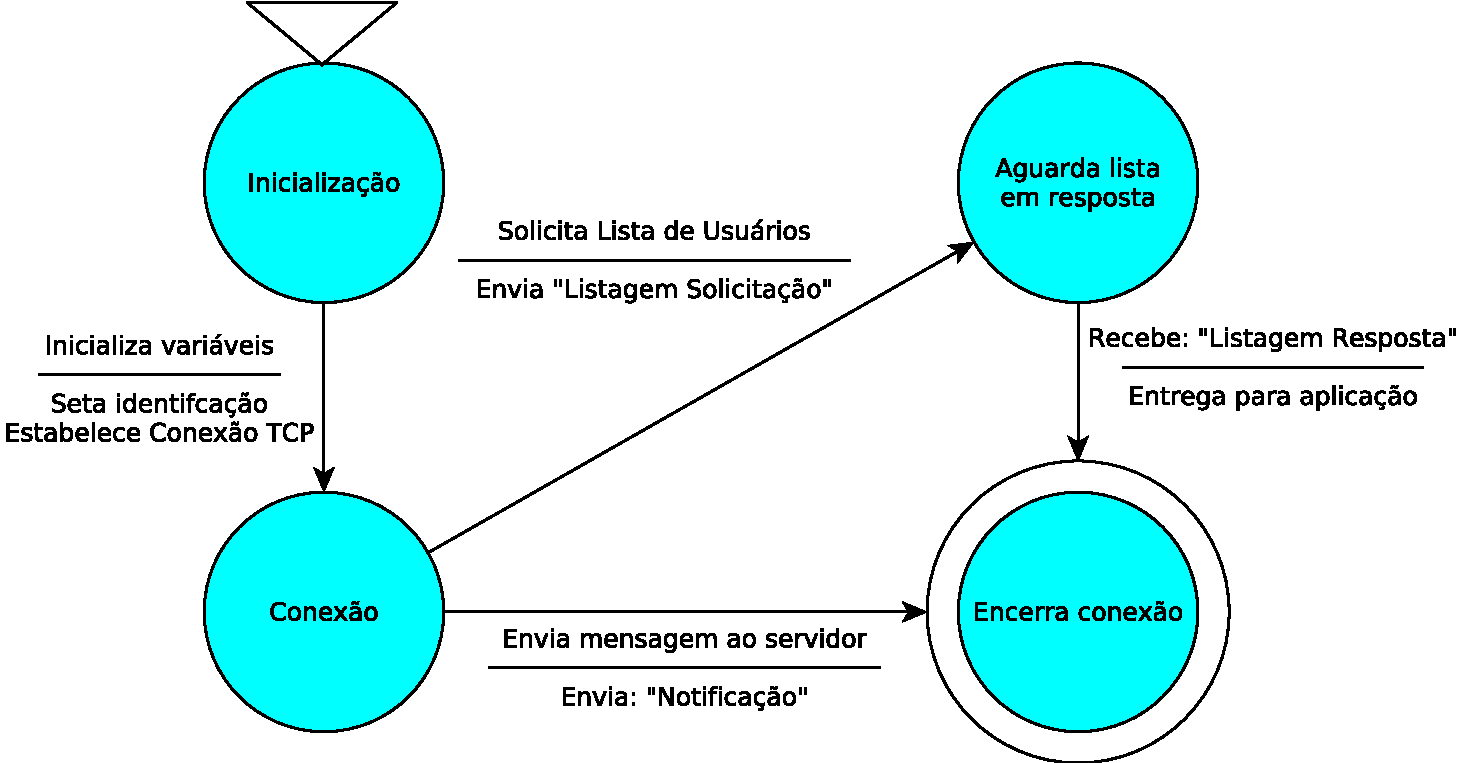
\includegraphics[width=1\textwidth]{images/Protocolo_Cliente_Emissor.pdf}
	\caption{Máquina de estados do Cliente Emissor.}
	\label{fig:Emissor}
\end{figure}

\begin{figure}%[ht]
	\centering
	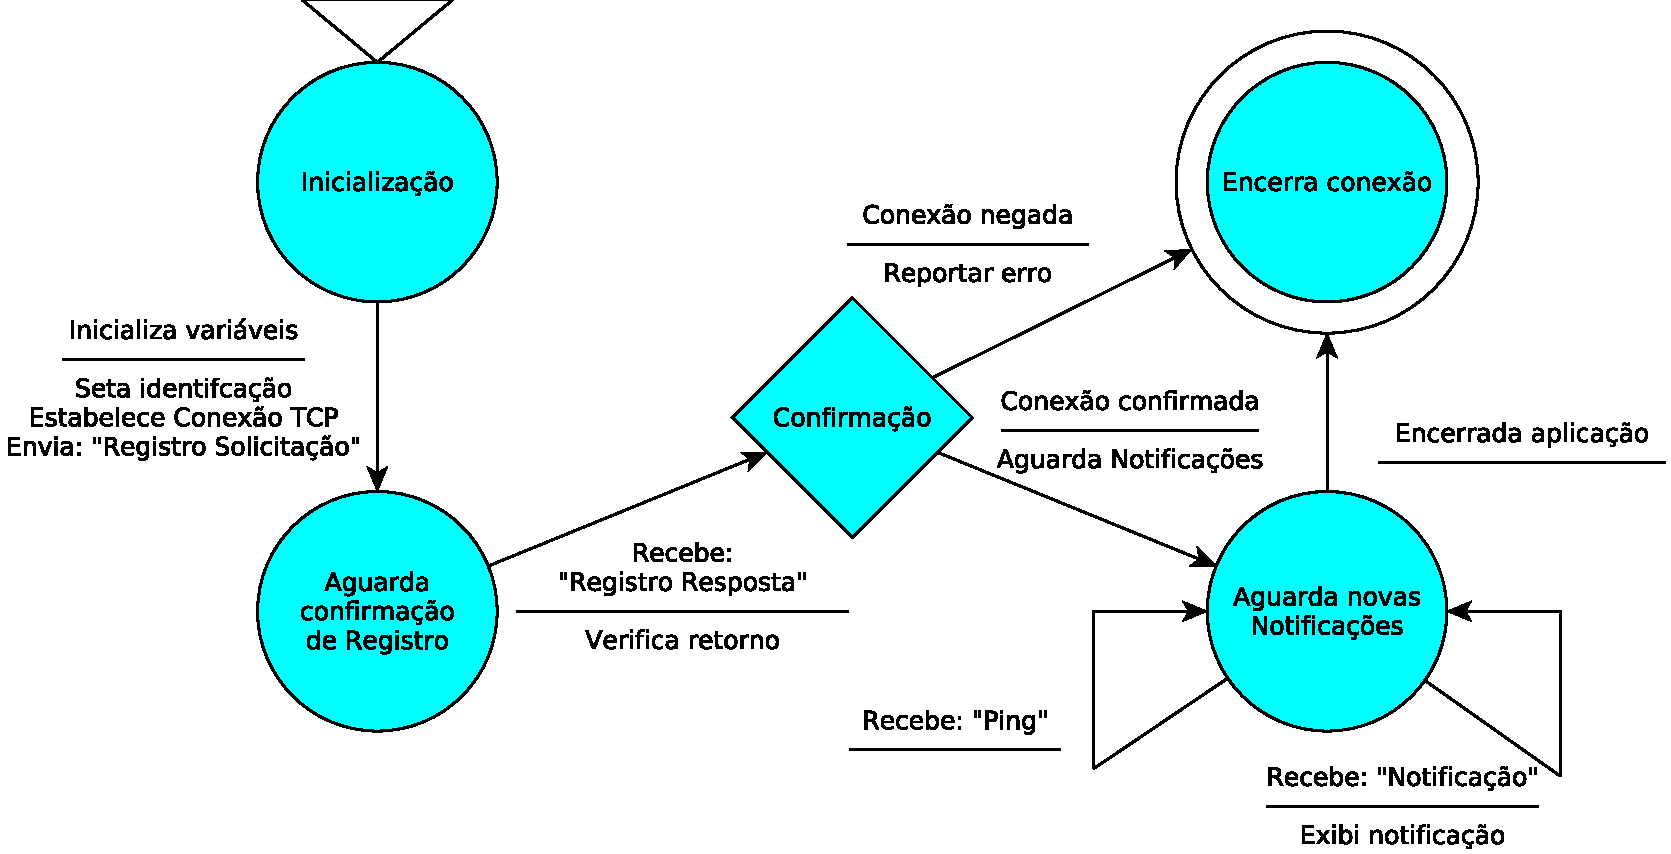
\includegraphics[width=1\textwidth]{images/Protocolo_Cliente_Receptor.pdf}
	\caption{Máquina de estados do Cliente Receptor.}
	\label{fig:Receptor}
\end{figure}

\begin{figure}%[ht]
	\centering
	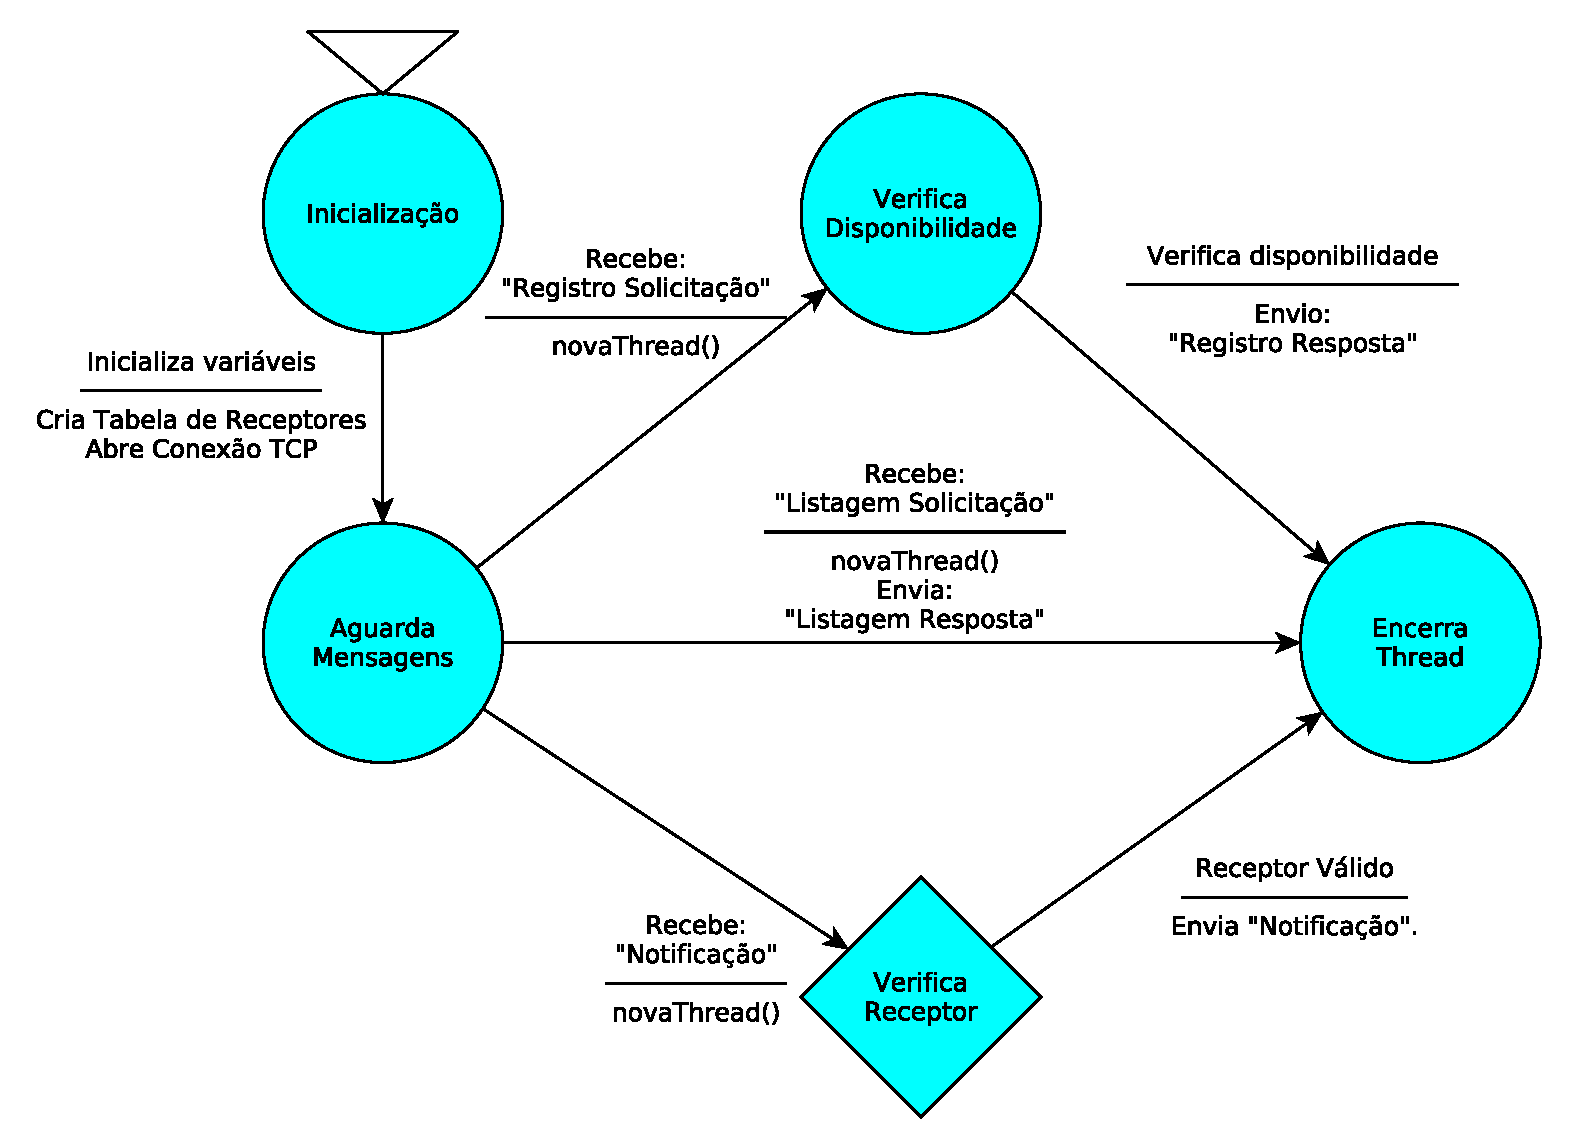
\includegraphics[width=1\textwidth]{images/Protocolo_Servidor.pdf}
	\caption{Máquina de estados do Servidor.}
	\label{fig:Servidor}
\end{figure}

%%=========================================================================================
\section{Mensagens}\label{sec:Mensagens}
%%=========================================================================================

O SSNR define quatro tipos de mensagens,
{\tt Notificação}, {\tt Listagem}, {\tt Registro} e {\tt Ping}.
Cada grupo de mensagens são usadas dentro de um mesmo contexto e compartilham o padrão de cabeçalho,
todo cabeçalho começa com um campo de {\bf Código} de 1 byte usado para identificar o tipo da mensagem.
Também é padronizado o tamanho dos "nomes", utilizados identificar usuários,
sendo estes uma sequência de 16 caracteres de 8 bits (16 bytes no total).

Mensagens do tipo {\tt Notificação} representam o principal tipo de mensagens enviadas no sistema.
Elas possuem um cabeçalho de 31 bytes e corpo variável:
\begin{itemize}
\item Cabeçalho:
	\begin{itemize}
	\item {\bf Código} - 1 byte;
	\item {\bf Tamanho} - 8 bytes;
	\item {\bf Código Receptor} - 2 bytes;
	\item {\bf Timestamp} - 4 bytes;
	\item {\bf Nome do Emissor} - 16 byte.
	\end{itemize}
\item Corpo:
	\begin{itemize}
	\item {\bf Texto} - Variável.
	\end{itemize}
\end{itemize}
O campo {\bf Código} representa o tipo da mensagem e deve sempre conter 078 (ASCII correspondente à 'N').
{\bf Tamanho} indica o tamanho total do {\bf Texto} da notificação.
{\bf Código Receptor} é o identificador do destinatário da notificação no servidor,
cada servidor pode então indexar até 65536 ($2^{16}$) receptores.
{\bf Timestamp} é o horário de envio da notificação no padrão Unix.
Por fim, o pacote contém o {\bf Nome do Emissor} seguido então pelo {\bf Texto} da notificação.

Mensagens do tipo {\tt Listagem} são usadas para informar emissores dos receptores disponíveis.
Possuem cabeçalho de 5 bytes e dois subtipos:
{\tt Solicitação}, que são enviadas por emissores;
e {\tt Resposta}, enviada por servidores.
Mensagens de {\tt Listagem} tem a seguinte organização:
\begin{itemize}
\item Cabeçalho:
	\begin{itemize}
	\item {\bf Código} - 1 byte;
	\item {\bf Número de usuários} - 2 bytes;
	\item {\bf Offset} - 2 bytes.
	\end{itemize}
\item Corpo em {\tt Solicitação}:
	\begin{itemize}
	\item {\bf Nome Emissor} - 16 bytes.
	\end{itemize}
\item Corpo em {\tt Resposta}:
	\begin{itemize}
	\item {\bf Lista de usuários} (Código e nome) - 18 bytes por par.
	\end{itemize}
\end{itemize}
O campo {\bf Código} deve sempre conter 076 (ASCII correspondente à 'L').
Na {\tt Solicitação}, o {\bf Número de usuários} contém o número máximo de usuários que se deseja receber;
já {\tt Resposta}, o campo contém o número de usuários retornados na mensagem.
O {\bf Offset} é usado na {\tt Solicitação} para controlar quais usuários pegar, se for maior ou igual ao número total de usuários no servidor a {\tt Resposta} é enviada sem nenhum usuário. 

Mensagens de {\tt Registro} são usados no início de uma nova conexão de um receptor ao servidor.
Estas mensagens possuem um tamanho total de 20 bytes e 2 subtipos:
{\tt Solicitação} e {\tt Resposta}.
\begin{itemize}
\item {\bf Código} - 1 byte.
\item {\bf Código Receptor} - 2 bytes.
\item {\bf Retorno} - 1 bytes.
\item {\bf Nome Receptor} - 16 bytes.
\end{itemize}
O campo {\bf Código} deve sempre conter 082 (ASCII correspondente à `R').
Na {\tt Solicitação} o campo {\bf Código Receptor} é usado como índice preferível,
e na {\tt Resposta} o índice ao qual o Receptor foi efetivamente alocado é informado no {\bf Código Receptor}.
O campo {\bf Retorno} na {\tt Confirmação} contem o resultado da operação,
{\bf Retorno} pode assumir os seguintes valores:
\begin{itemize}
\item 0 - Conexão bem sucedida no endereço requirido.
\item 1 - Conexão bem sucedida no endereço retornado em {\bf Código Receptor}
\item 2 - Conexão recusada, servidor cheio.
\item 4 - Conexão recusada, servidor lista negra.
\item 128 - Erro não informado.
\end{itemize}

Por fim, a mensagem de {\tt Ping} consiste apenas da repetição de dois bytes com valor 80
(código ASCII para 'P').
Mensagens de Ping são enviadas pelo servidor a todos os Receptores conectados sempre que
há necessidade de conferir se a conexão ainda é válida.
{\tt Ping} é enviado sempre que um novo registro é requirido para verificar disponibilidade de índices;
ele também é enviado quando uma listagem é requirida para evitar a listagem de receptores desconectados.

%%=========================================================================================
\section{Conclusão}\label{sec:Conclusao}
%%=========================================================================================

O Sistema Simples de Notificação Remota é um protocolo de notificações distribuídas que
permite uma implementação simples de clientes,
especializando-os nas funções de emissor ou receptor.
Aplicações que disponham de mais robustez podem implementar ambos os protocolos de cliente se assim desejarem.

Para um exemplo de uso deste protocolo então propomos três aplicações diferentes:
(1) O Servidor, de uso como descrito no protocolo.
(2) Uma aplicação de terminal para {\it Desktops} que pode enviar notificações.
(3) E um aplicativo para Celular que apenas recebe notificações.
Tomando como cenário então vários {\it Desktops} que possuem a implementação mencionada
e que computam programas que levam tempo arbitrário para terminar.
É possível então, com um pouco de habilidade em {\it Shell Script},
fazer com que sempre que um programa terminar a execução,
uma notificação seja enviada para o Celular com tal aplicativo indicando:
a máquina que enviou a notificação (no campo {\bf Nome Emissor} da Notificação),
e parte da saída padrão ou saída de erro do programa (no campo {\bf Texto}).

\end{document}
